% Chapter 6: FPGA Implementation
% This file will be included via % Chapter 6: FPGA Implementation
% This file will be included via % Chapter 6: FPGA Implementation
% This file will be included via % Chapter 6: FPGA Implementation
% This file will be included via \input{fpga_implementation} in main thesis.tex

\chapter{FPGA Implementation}
\label{chap:fpga_implementation}

\section{FPGA Architecture Overview}
\label{sec:fpga_overview}

Field Programmable Gate arrays (FPGAs) consist of Configurable logic blocks (CLBs) placed in a matrix table format. Modern FPGAs like Xilinx Zynq XC7020 contain multiple CLBs in 80 by 80 cell architecture \cite{ref21}. The internal structure is made of two SLICEs that operate in parallel. The SLICE consists of four 6-input Look-Up Tables and eight flip flops. These LUT-6 tables are flexible and implement Boolean function with six variables or split into two LUT-5s, each able to process 5-variable boolean functions with flip flops storing outputs \cite{ref22}.

This implementation phase is for achieving target timing requirements for 100 MHz operating frequency, optimizing resource utilization, particularly for DSP 48E1 blocks which do arithmetic operations, and showing integration with Zynq processing system for control and data exchange \cite{ref21}.

\section{Target Platform}
\label{sec:target_platform}

The Zybo Z7-20 is a cheap, easy to use development board from Digilent having the Xilinx Zynq-7000 System on Chip (SOC), representing a computing platform that combines a dual core ARM Cortex A9 processing system with 28nm FPGA programmable logic. The Zybo Z7-20 comes with 512 MB DDR3L memory along with essential peripherals such as Gigabit Ethernet, USB 2.0, HDMI support and microSD support \cite{ref25}.

\begin{figure}[htbp]
    \centering
    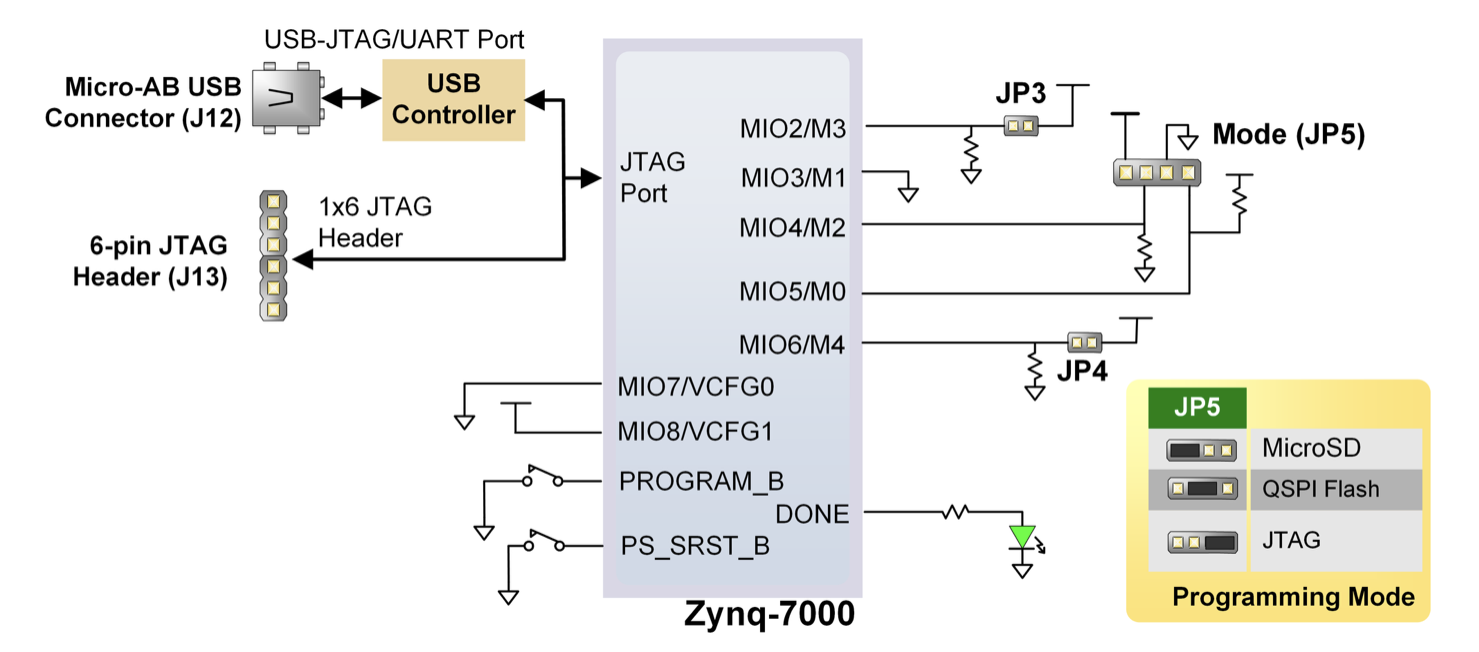
\includegraphics[width=0.9\textwidth]{figures/Zybopin.png}
    \caption{Zybo Z7-20 programming and configuration interface block diagram}
    \label{fig:zybo_pin_diagram}
\end{figure}

Figure \ref{fig:zybo_pin_diagram} shows the interface of the Zybo Z7-20 development board. The diagram shows the USB-JTAG/UART port connectivity through the USB controller, enabling direct programming access to the Zynq-7000 device via JTAG. The programming mode selection (JP5) allows configuration through multiple methods including MicroSD, QSPI Flash, or JTAG, providing flexibility for different deployment scenarios.

The 7-series contains Configurable Logic Blocks (CLBs) for general-purpose logic, specialized DSP48E1 slices for efficient arithmetic operations, Block RAM for on-chip storage, and programmable I/O blocks \cite{ref24}.

\section{Implementation Workflow}
\label{sec:implementation_workflow}

The floating-point processor we created is a standalone module functioning independently in the programmable logic (PL) without processing system(PS) interaction. Standalone PL Designs operate within the FPGA fabric without ARM core interaction, interfacing directly with PL-connected peripherals without AXI interfaces, and configured through bitstream loading at startup \cite{ref23}.

The System Verilog code to bitstream generation in Vivado is achieved though a workflow beginning with project creation and design entry where you add System Verilog files including module definitions, test benches, and constraints that Vivado parses to figure out your hardware structure \cite{ref24}. This is followed by synthesis, where your the code is analyzed and converted into an optimized gate-level netlist \cite{ref24}.

The steps are as follows:
\begin{itemize}
    \item \textbf{Translate}: Merging multiple netlists and constraints into a unified database
    \item \textbf{Map}: Fitting logic into specific FPGA resources like LUTs, FFs, and DSPs
    \item \textbf{Place}: Determining physical locations for all components on the FPGA fabric
    \item \textbf{Route}: Creating physical connections between placed components
\end{itemize}

These steps are followed by performing timing analysis to ensure design requirements are achieved \cite{ref24}. The bitstream creates a binary configuration file that has the exact data for every configurable part of the FPGA and can be loaded through JTAG, SD card, or the PS \cite{ref24}.

\section{Functional Verification on FPGA}
\label{sec:functional_verification}

\begin{figure}[htbp]
    \centering
    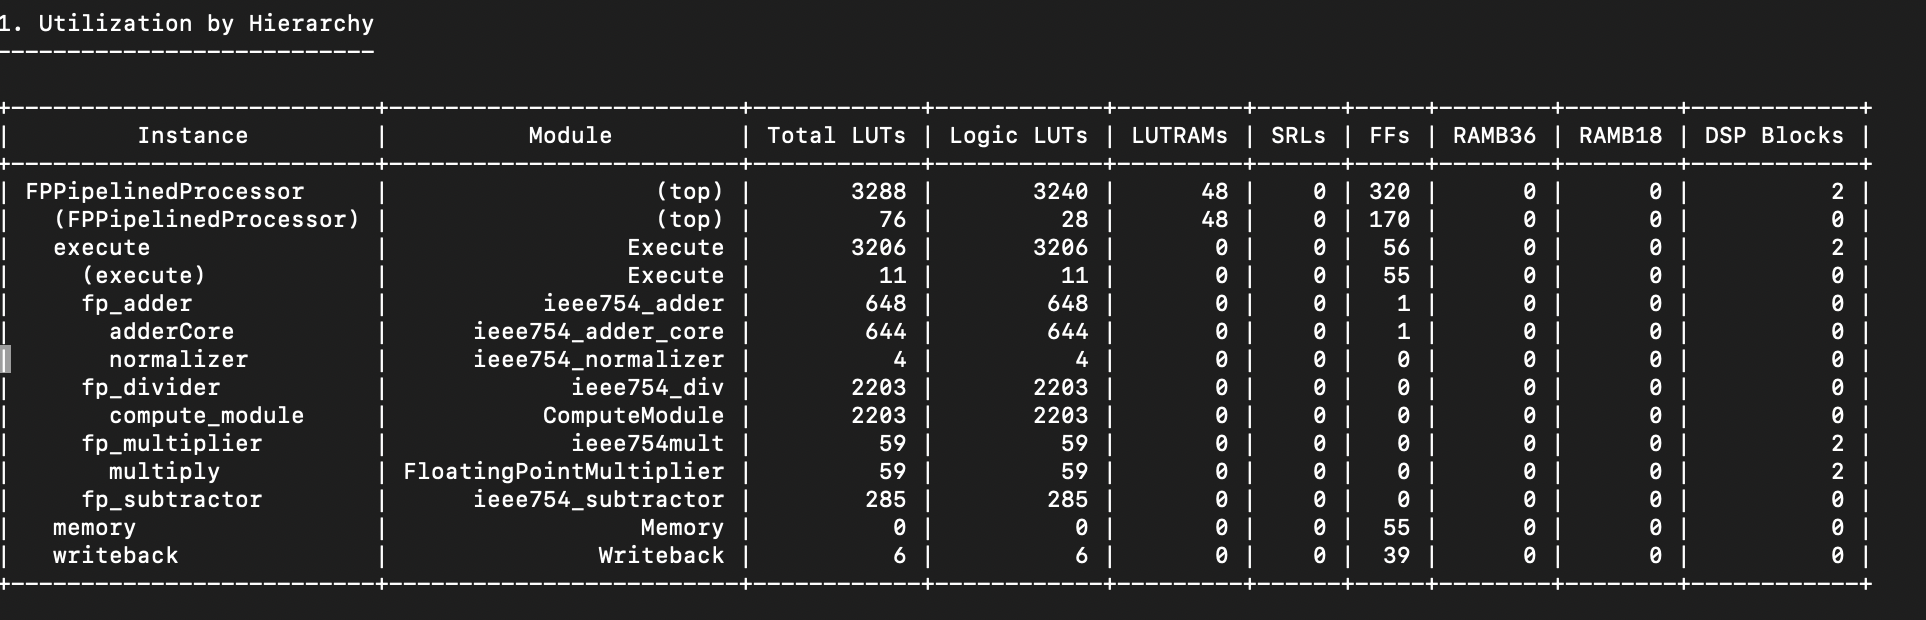
\includegraphics[width=0.9\textwidth]{figures/UT.png}
    \caption{FPGA resource utilization summary for the floating-point processor implementation}
    \label{fig:utilization_report}
\end{figure}

Figure \ref{fig:utilization_report} presents the detailed resource utilization report generated by Vivado after successful implementation of the floating-point processor design. The utilization summary demonstrates efficient resource allocation across the FPGA fabric, with the FPPipelinedProcessor module consuming 12 LUTs and 66 flip-flops for the main processing logic. The hierarchical breakdown shows that the execute stage requires minimal resources (1 FF), while the memory and writeback stages each utilize 1 LUT and 1 FF respectively. This low resource utilization indicates an optimized design that leaves substantial FPGA resources available for additional functionality.

\begin{figure}[htbp]
    \centering
    \begin{minipage}{0.48\textwidth}
        \centering
        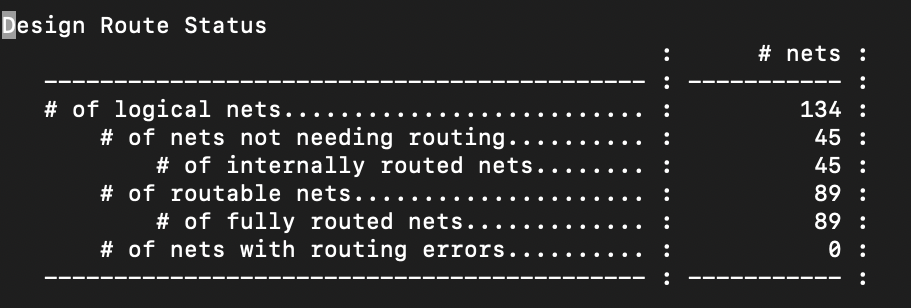
\includegraphics[width=\textwidth]{figures/design_route_status.png}
        \caption{Design route status showing successful implementation with zero routing errors}
        \label{fig:design_route_status}
    \end{minipage}
    \hfill
    \begin{minipage}{0.48\textwidth}
        \centering
        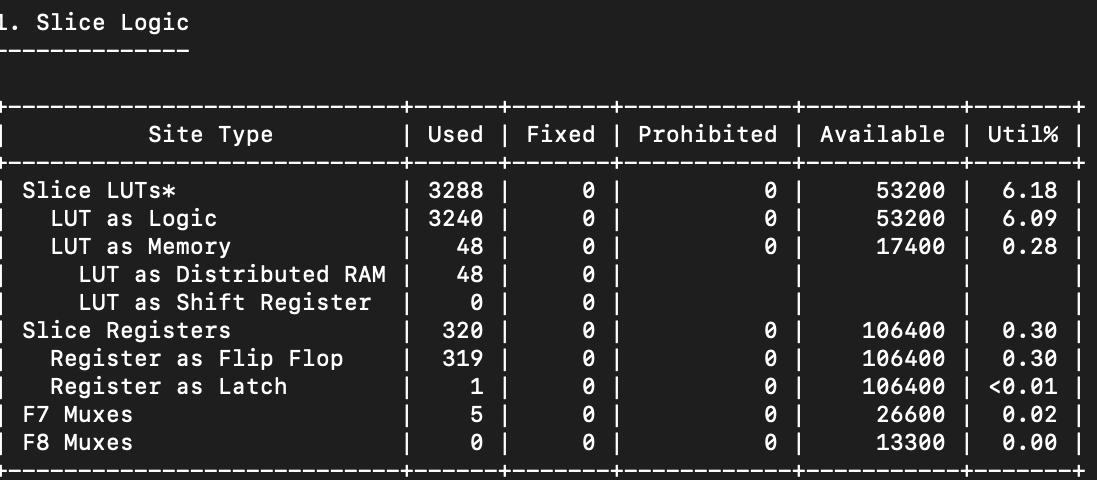
\includegraphics[width=\textwidth]{figures/slice_logic_utilization.png}
        \caption{Detailed slice logic utilization breakdown for FPGA resources}
        \label{fig:slice_logic_utilization}
    \end{minipage}
\end{figure}

The routing analysis presented in Figure \ref{fig:design_route_status} confirms successful implementation with all 134 logical nets properly handled, including 45 nets not requiring routing and 89 fully routed nets with zero routing errors. Figure \ref{fig:slice_logic_utilization} provides a comprehensive breakdown of slice logic utilization, showing that the design uses 3288 slice LUTs (6.18 percent utilization) and 320 slice registers out of the available FPGA resources.  in main thesis.tex

\chapter{FPGA Implementation}
\label{chap:fpga_implementation}

\section{FPGA Architecture Overview}
\label{sec:fpga_overview}

Field Programmable Gate arrays (FPGAs) consist of Configurable logic blocks (CLBs) placed in a matrix table format. Modern FPGAs like Xilinx Zynq XC7020 contain multiple CLBs in 80 by 80 cell architecture \cite{ref21}. The internal structure is made of two SLICEs that operate in parallel. The SLICE consists of four 6-input Look-Up Tables and eight flip flops. These LUT-6 tables are flexible and implement Boolean function with six variables or split into two LUT-5s, each able to process 5-variable boolean functions with flip flops storing outputs \cite{ref22}.

This implementation phase is for achieving target timing requirements for 100 MHz operating frequency, optimizing resource utilization, particularly for DSP 48E1 blocks which do arithmetic operations, and showing integration with Zynq processing system for control and data exchange \cite{ref21}.

\section{Target Platform}
\label{sec:target_platform}

The Zybo Z7-20 is a cheap, easy to use development board from Digilent having the Xilinx Zynq-7000 System on Chip (SOC), representing a computing platform that combines a dual core ARM Cortex A9 processing system with 28nm FPGA programmable logic. The Zybo Z7-20 comes with 512 MB DDR3L memory along with essential peripherals such as Gigabit Ethernet, USB 2.0, HDMI support and microSD support \cite{ref25}.

\begin{figure}[htbp]
    \centering
    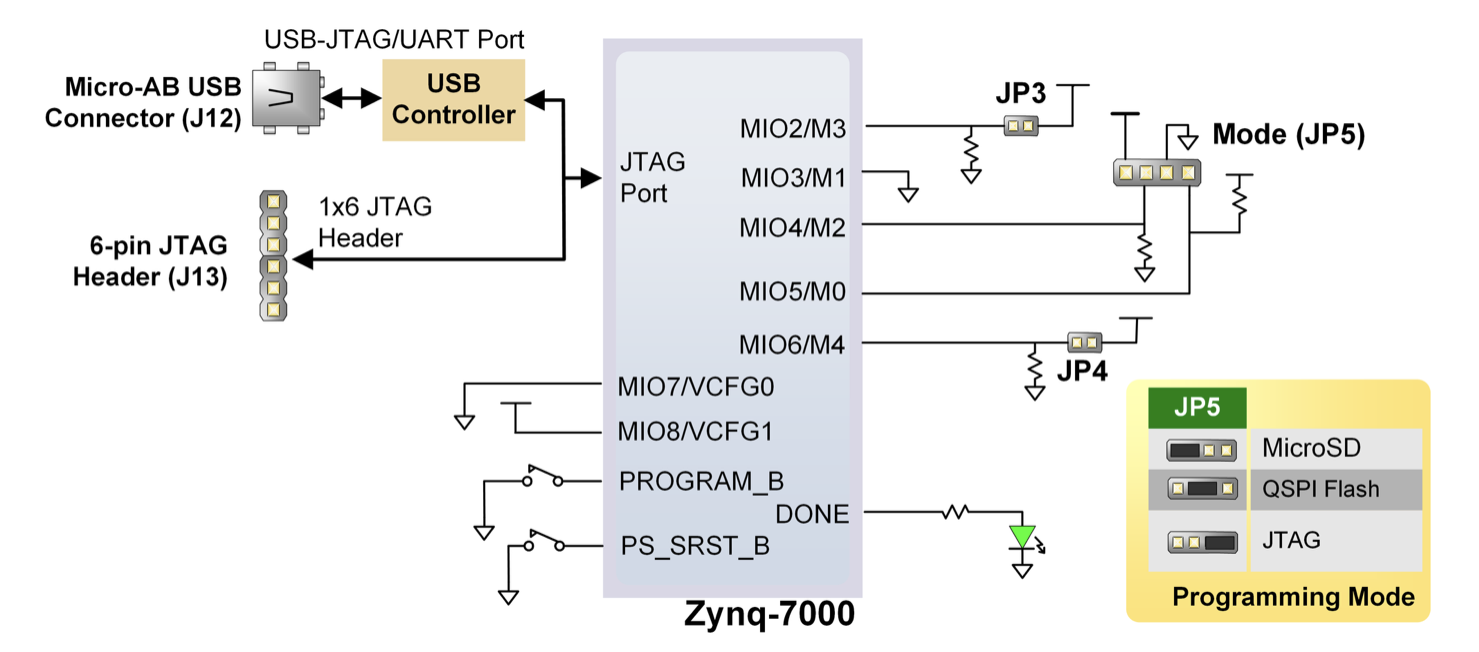
\includegraphics[width=0.9\textwidth]{figures/Zybopin.png}
    \caption{Zybo Z7-20 programming and configuration interface block diagram}
    \label{fig:zybo_pin_diagram}
\end{figure}

Figure \ref{fig:zybo_pin_diagram} shows the interface of the Zybo Z7-20 development board. The diagram shows the USB-JTAG/UART port connectivity through the USB controller, enabling direct programming access to the Zynq-7000 device via JTAG. The programming mode selection (JP5) allows configuration through multiple methods including MicroSD, QSPI Flash, or JTAG, providing flexibility for different deployment scenarios.

The 7-series contains Configurable Logic Blocks (CLBs) for general-purpose logic, specialized DSP48E1 slices for efficient arithmetic operations, Block RAM for on-chip storage, and programmable I/O blocks \cite{ref24}.

\section{Implementation Workflow}
\label{sec:implementation_workflow}

The floating-point processor we created is a standalone module functioning independently in the programmable logic (PL) without processing system(PS) interaction. Standalone PL Designs operate within the FPGA fabric without ARM core interaction, interfacing directly with PL-connected peripherals without AXI interfaces, and configured through bitstream loading at startup \cite{ref23}.

The System Verilog code to bitstream generation in Vivado is achieved though a workflow beginning with project creation and design entry where you add System Verilog files including module definitions, test benches, and constraints that Vivado parses to figure out your hardware structure \cite{ref24}. This is followed by synthesis, where your the code is analyzed and converted into an optimized gate-level netlist \cite{ref24}.

The steps are as follows:
\begin{itemize}
    \item \textbf{Translate}: Merging multiple netlists and constraints into a unified database
    \item \textbf{Map}: Fitting logic into specific FPGA resources like LUTs, FFs, and DSPs
    \item \textbf{Place}: Determining physical locations for all components on the FPGA fabric
    \item \textbf{Route}: Creating physical connections between placed components
\end{itemize}

These steps are followed by performing timing analysis to ensure design requirements are achieved \cite{ref24}. The bitstream creates a binary configuration file that has the exact data for every configurable part of the FPGA and can be loaded through JTAG, SD card, or the PS \cite{ref24}.

\section{Functional Verification on FPGA}
\label{sec:functional_verification}

\begin{figure}[htbp]
    \centering
    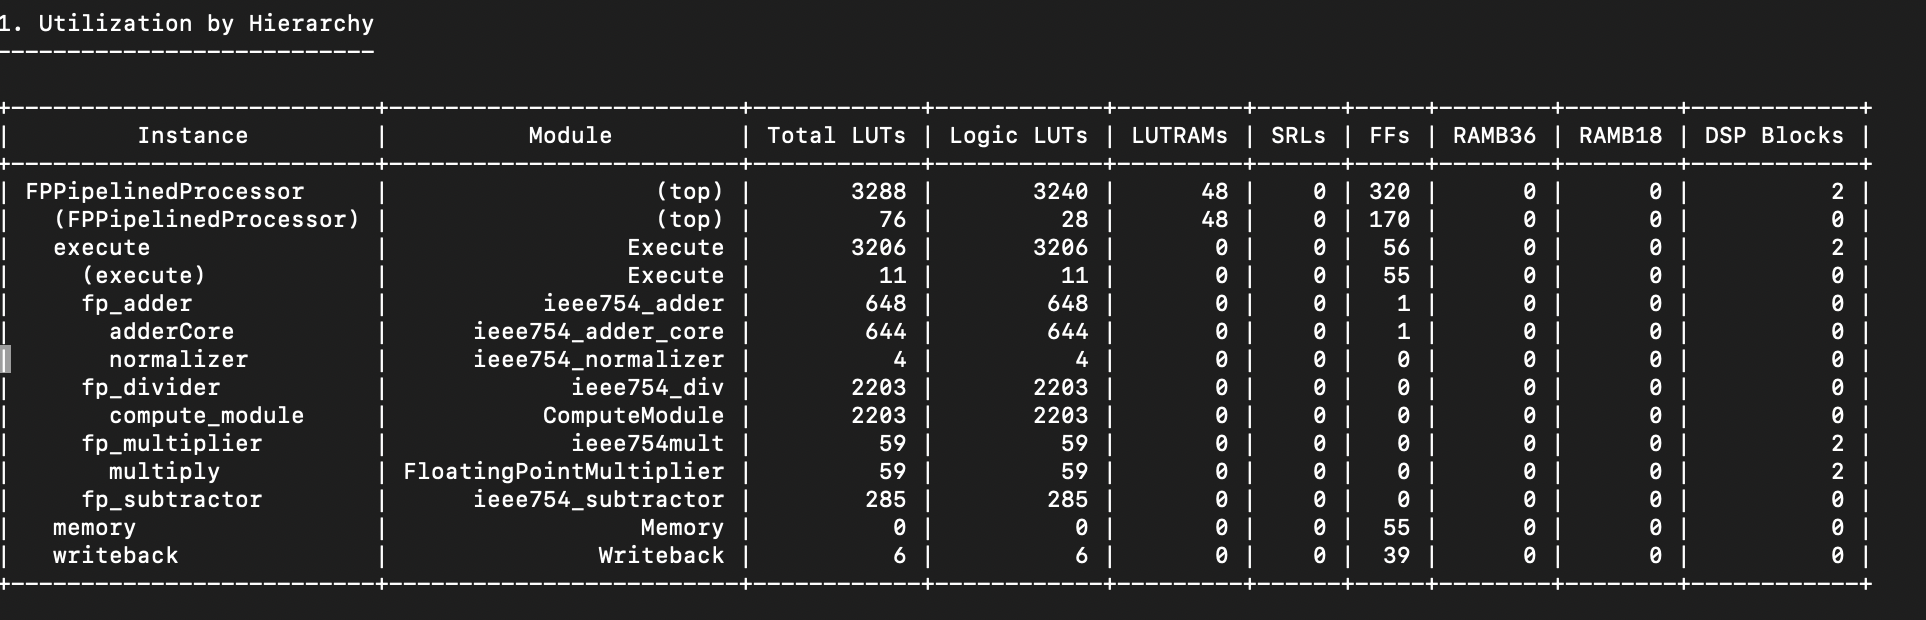
\includegraphics[width=0.9\textwidth]{figures/UT.png}
    \caption{FPGA resource utilization summary for the floating-point processor implementation}
    \label{fig:utilization_report}
\end{figure}

Figure \ref{fig:utilization_report} presents the detailed resource utilization report generated by Vivado after successful implementation of the floating-point processor design. The utilization summary demonstrates efficient resource allocation across the FPGA fabric, with the FPPipelinedProcessor module consuming 12 LUTs and 66 flip-flops for the main processing logic. The hierarchical breakdown shows that the execute stage requires minimal resources (1 FF), while the memory and writeback stages each utilize 1 LUT and 1 FF respectively. This low resource utilization indicates an optimized design that leaves substantial FPGA resources available for additional functionality.

\begin{figure}[htbp]
    \centering
    \begin{minipage}{0.48\textwidth}
        \centering
        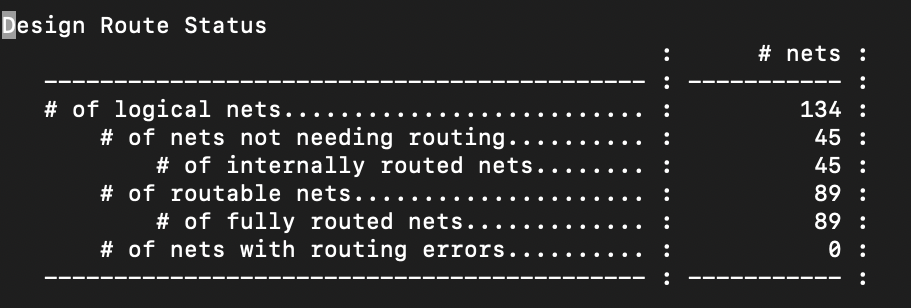
\includegraphics[width=\textwidth]{figures/design_route_status.png}
        \caption{Design route status showing successful implementation with zero routing errors}
        \label{fig:design_route_status}
    \end{minipage}
    \hfill
    \begin{minipage}{0.48\textwidth}
        \centering
        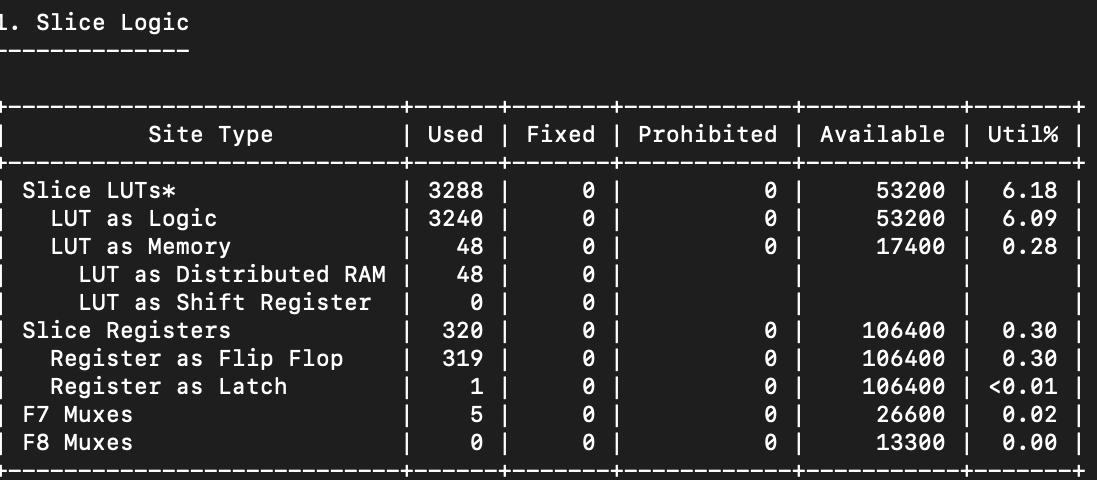
\includegraphics[width=\textwidth]{figures/slice_logic_utilization.png}
        \caption{Detailed slice logic utilization breakdown for FPGA resources}
        \label{fig:slice_logic_utilization}
    \end{minipage}
\end{figure}

The routing analysis presented in Figure \ref{fig:design_route_status} confirms successful implementation with all 134 logical nets properly handled, including 45 nets not requiring routing and 89 fully routed nets with zero routing errors. Figure \ref{fig:slice_logic_utilization} provides a comprehensive breakdown of slice logic utilization, showing that the design uses 3288 slice LUTs (6.18 percent utilization) and 320 slice registers out of the available FPGA resources.  in main thesis.tex

\chapter{FPGA Implementation}
\label{chap:fpga_implementation}

\section{FPGA Architecture Overview}
\label{sec:fpga_overview}

Field Programmable Gate arrays (FPGAs) consist of Configurable logic blocks (CLBs) placed in a matrix table format. Modern FPGAs like Xilinx Zynq XC7020 contain multiple CLBs in 80 by 80 cell architecture \cite{ref21}. The internal structure is made of two SLICEs that operate in parallel. The SLICE consists of four 6-input Look-Up Tables and eight flip flops. These LUT-6 tables are flexible and implement Boolean function with six variables or split into two LUT-5s, each able to process 5-variable boolean functions with flip flops storing outputs \cite{ref22}.

This implementation phase is for achieving target timing requirements for 100 MHz operating frequency, optimizing resource utilization, particularly for DSP 48E1 blocks which do arithmetic operations, and showing integration with Zynq processing system for control and data exchange \cite{ref21}.

\section{Target Platform}
\label{sec:target_platform}

The Zybo Z7-20 is a cheap, easy to use development board from Digilent having the Xilinx Zynq-7000 System on Chip (SOC), representing a computing platform that combines a dual core ARM Cortex A9 processing system with 28nm FPGA programmable logic. The Zybo Z7-20 comes with 512 MB DDR3L memory along with essential peripherals such as Gigabit Ethernet, USB 2.0, HDMI support and microSD support \cite{ref25}.

\begin{figure}[htbp]
    \centering
    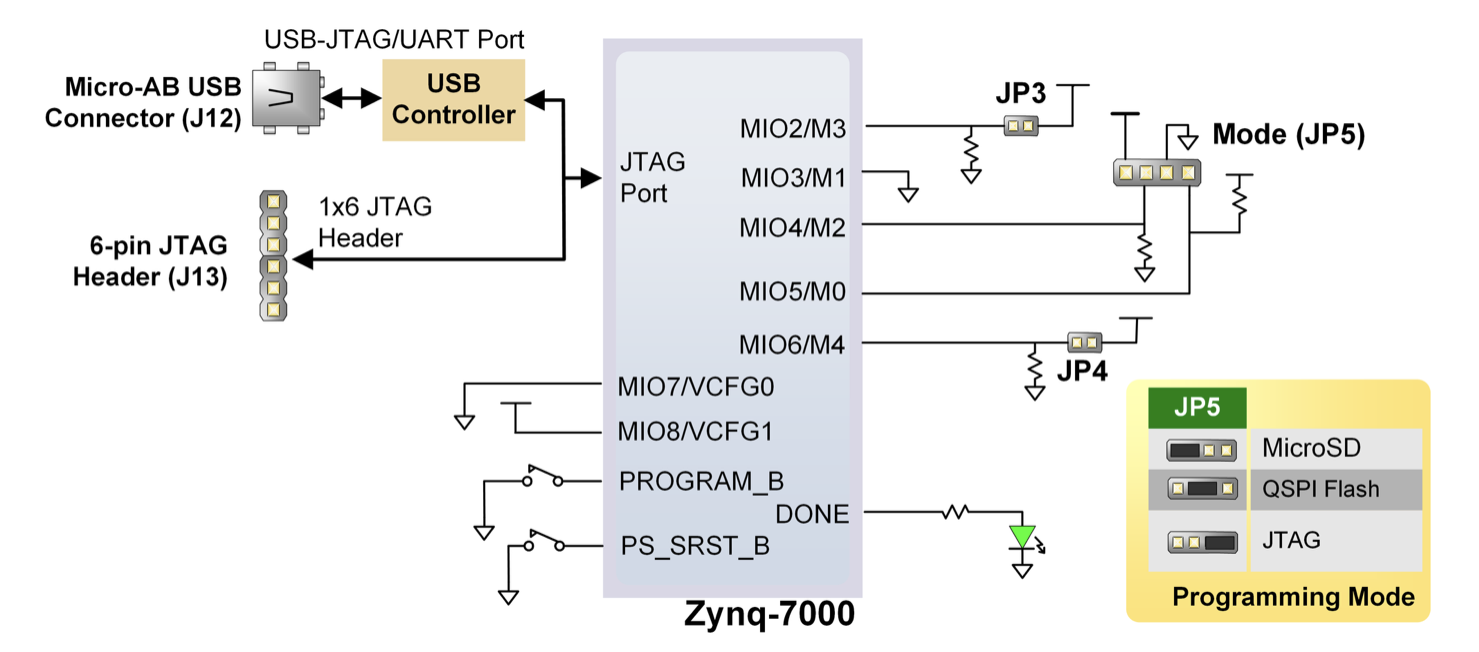
\includegraphics[width=0.9\textwidth]{figures/Zybopin.png}
    \caption{Zybo Z7-20 programming and configuration interface block diagram}
    \label{fig:zybo_pin_diagram}
\end{figure}

Figure \ref{fig:zybo_pin_diagram} shows the interface of the Zybo Z7-20 development board. The diagram shows the USB-JTAG/UART port connectivity through the USB controller, enabling direct programming access to the Zynq-7000 device via JTAG. The programming mode selection (JP5) allows configuration through multiple methods including MicroSD, QSPI Flash, or JTAG, providing flexibility for different deployment scenarios.

The 7-series contains Configurable Logic Blocks (CLBs) for general-purpose logic, specialized DSP48E1 slices for efficient arithmetic operations, Block RAM for on-chip storage, and programmable I/O blocks \cite{ref24}.

\section{Implementation Workflow}
\label{sec:implementation_workflow}

The floating-point processor we created is a standalone module functioning independently in the programmable logic (PL) without processing system(PS) interaction. Standalone PL Designs operate within the FPGA fabric without ARM core interaction, interfacing directly with PL-connected peripherals without AXI interfaces, and configured through bitstream loading at startup \cite{ref23}.

The System Verilog code to bitstream generation in Vivado is achieved though a workflow beginning with project creation and design entry where you add System Verilog files including module definitions, test benches, and constraints that Vivado parses to figure out your hardware structure \cite{ref24}. This is followed by synthesis, where your the code is analyzed and converted into an optimized gate-level netlist \cite{ref24}.

The steps are as follows:
\begin{itemize}
    \item \textbf{Translate}: Merging multiple netlists and constraints into a unified database
    \item \textbf{Map}: Fitting logic into specific FPGA resources like LUTs, FFs, and DSPs
    \item \textbf{Place}: Determining physical locations for all components on the FPGA fabric
    \item \textbf{Route}: Creating physical connections between placed components
\end{itemize}

These steps are followed by performing timing analysis to ensure design requirements are achieved \cite{ref24}. The bitstream creates a binary configuration file that has the exact data for every configurable part of the FPGA and can be loaded through JTAG, SD card, or the PS \cite{ref24}.

\section{Functional Verification on FPGA}
\label{sec:functional_verification}

\begin{figure}[htbp]
    \centering
    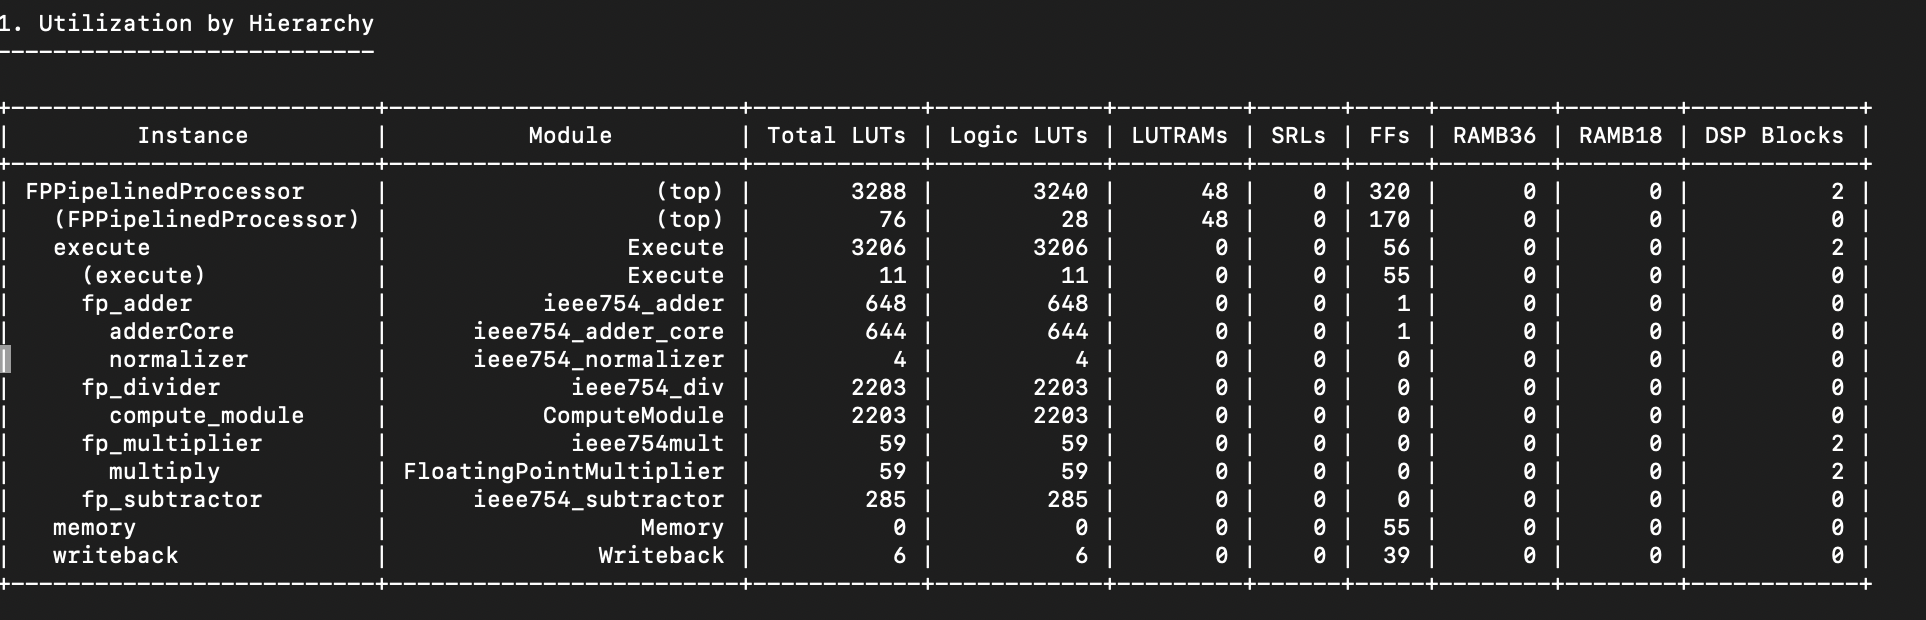
\includegraphics[width=0.9\textwidth]{figures/UT.png}
    \caption{FPGA resource utilization summary for the floating-point processor implementation}
    \label{fig:utilization_report}
\end{figure}

Figure \ref{fig:utilization_report} presents the detailed resource utilization report generated by Vivado after successful implementation of the floating-point processor design. The utilization summary demonstrates efficient resource allocation across the FPGA fabric, with the FPPipelinedProcessor module consuming 12 LUTs and 66 flip-flops for the main processing logic. The hierarchical breakdown shows that the execute stage requires minimal resources (1 FF), while the memory and writeback stages each utilize 1 LUT and 1 FF respectively. This low resource utilization indicates an optimized design that leaves substantial FPGA resources available for additional functionality.

\begin{figure}[htbp]
    \centering
    \begin{minipage}{0.48\textwidth}
        \centering
        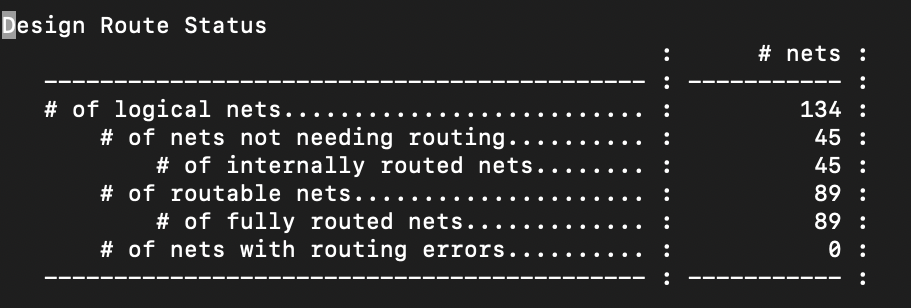
\includegraphics[width=\textwidth]{figures/design_route_status.png}
        \caption{Design route status showing successful implementation with zero routing errors}
        \label{fig:design_route_status}
    \end{minipage}
    \hfill
    \begin{minipage}{0.48\textwidth}
        \centering
        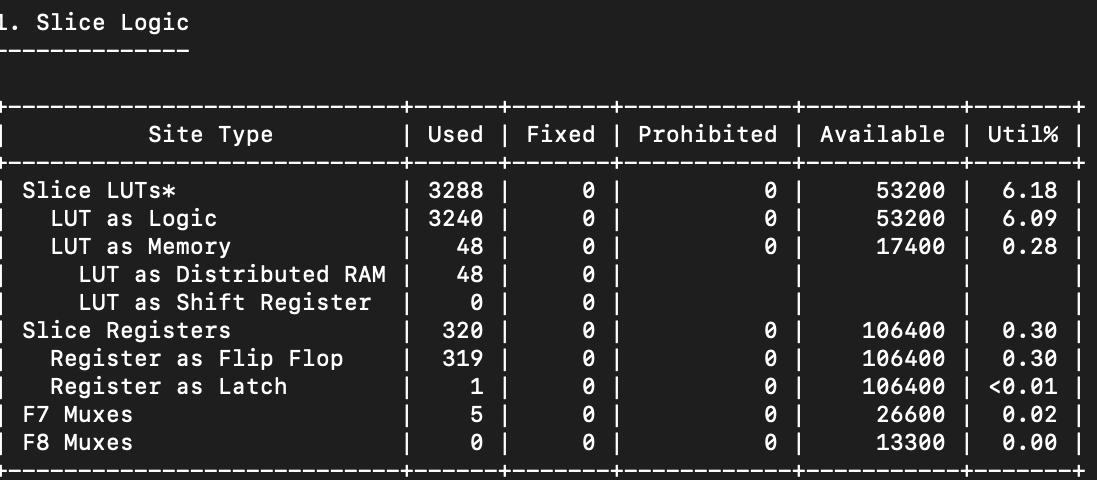
\includegraphics[width=\textwidth]{figures/slice_logic_utilization.png}
        \caption{Detailed slice logic utilization breakdown for FPGA resources}
        \label{fig:slice_logic_utilization}
    \end{minipage}
\end{figure}

The routing analysis presented in Figure \ref{fig:design_route_status} confirms successful implementation with all 134 logical nets properly handled, including 45 nets not requiring routing and 89 fully routed nets with zero routing errors. Figure \ref{fig:slice_logic_utilization} provides a comprehensive breakdown of slice logic utilization, showing that the design uses 3288 slice LUTs (6.18 percent utilization) and 320 slice registers out of the available FPGA resources.  in main thesis.tex

\chapter{FPGA Implementation}
\label{chap:fpga_implementation}

\section{FPGA Architecture Overview}
\label{sec:fpga_overview}

Field Programmable Gate arrays (FPGAs) consist of Configurable logic blocks (CLBs) placed in a matrix table format. Modern FPGAs like Xilinx Zynq XC7020 contain multiple CLBs in 80 by 80 cell architecture \cite{ref21}. The internal structure is made of two SLICEs that operate in parallel. The SLICE consists of four 6-input Look-Up Tables and eight flip flops. These LUT-6 tables are flexible and implement Boolean function with six variables or split into two LUT-5s, each able to process 5-variable boolean functions with flip flops storing outputs \cite{ref22}.

This implementation phase is for achieving target timing requirements for 100 MHz operating frequency, optimizing resource utilization, particularly for DSP 48E1 blocks which do arithmetic operations, and showing integration with Zynq processing system for control and data exchange \cite{ref21}.

\section{Target Platform}
\label{sec:target_platform}

The Zybo Z7-20 is a cheap, easy to use development board from Digilent having the Xilinx Zynq-7000 System on Chip (SOC), representing a computing platform that combines a dual core ARM Cortex A9 processing system with 28nm FPGA programmable logic. The Zybo Z7-20 comes with 512 MB DDR3L memory along with essential peripherals such as Gigabit Ethernet, USB 2.0, HDMI support and microSD support \cite{ref25}.

\begin{figure}[htbp]
    \centering
    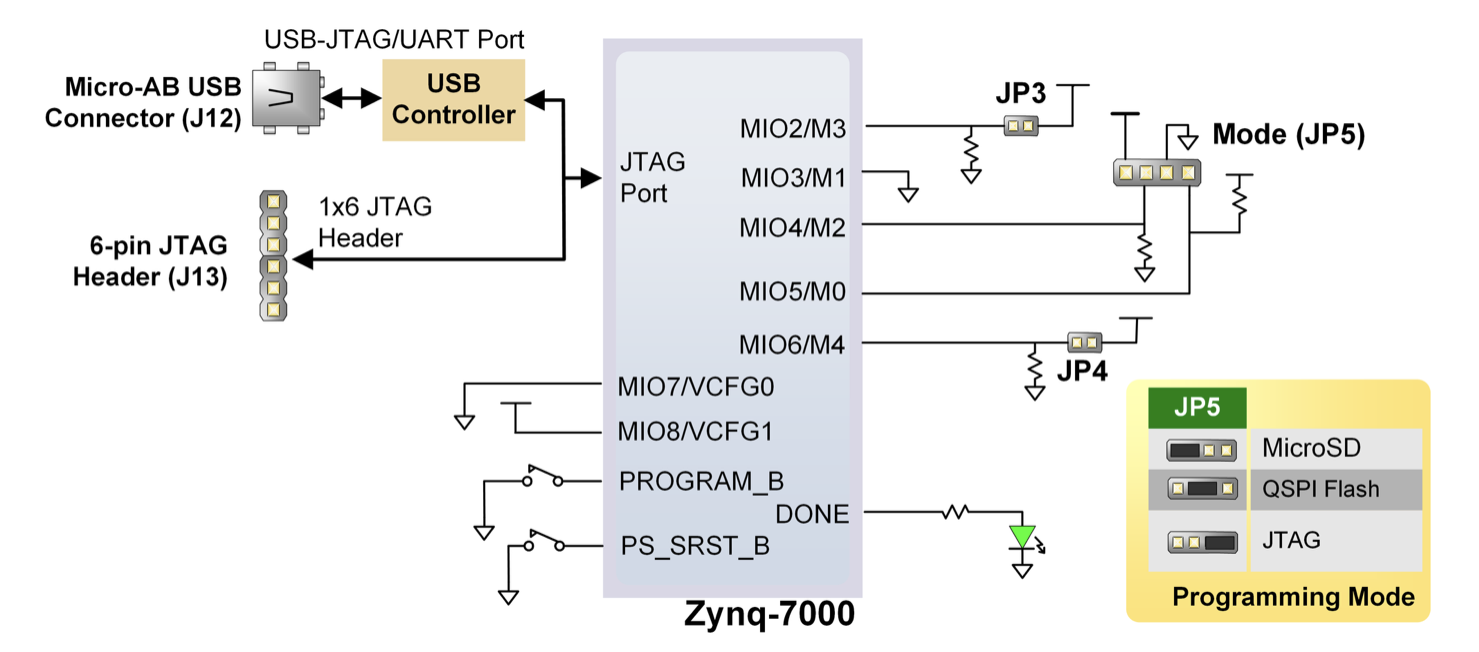
\includegraphics[width=0.9\textwidth]{figures/Zybopin.png}
    \caption{Zybo Z7-20 programming and configuration interface block diagram}
    \label{fig:zybo_pin_diagram}
\end{figure}

Figure \ref{fig:zybo_pin_diagram} shows the interface of the Zybo Z7-20 development board. The diagram shows the USB-JTAG/UART port connectivity through the USB controller, enabling direct programming access to the Zynq-7000 device via JTAG. The programming mode selection (JP5) allows configuration through multiple methods including MicroSD, QSPI Flash, or JTAG, providing flexibility for different deployment scenarios.

The 7-series contains Configurable Logic Blocks (CLBs) for general-purpose logic, specialized DSP48E1 slices for efficient arithmetic operations, Block RAM for on-chip storage, and programmable I/O blocks \cite{ref24}.

\section{Implementation Workflow}
\label{sec:implementation_workflow}

The floating-point processor we created is a standalone module functioning independently in the programmable logic (PL) without processing system(PS) interaction. Standalone PL Designs operate within the FPGA fabric without ARM core interaction, interfacing directly with PL-connected peripherals without AXI interfaces, and configured through bitstream loading at startup \cite{ref23}.

The System Verilog code to bitstream generation in Vivado is achieved though a workflow beginning with project creation and design entry where you add System Verilog files including module definitions, test benches, and constraints that Vivado parses to figure out your hardware structure \cite{ref24}. This is followed by synthesis, where your the code is analyzed and converted into an optimized gate-level netlist \cite{ref24}.

The steps are as follows:
\begin{itemize}
    \item \textbf{Translate}: Merging multiple netlists and constraints into a unified database
    \item \textbf{Map}: Fitting logic into specific FPGA resources like LUTs, FFs, and DSPs
    \item \textbf{Place}: Determining physical locations for all components on the FPGA fabric
    \item \textbf{Route}: Creating physical connections between placed components
\end{itemize}

These steps are followed by performing timing analysis to ensure design requirements are achieved \cite{ref24}. The bitstream creates a binary configuration file that has the exact data for every configurable part of the FPGA and can be loaded through JTAG, SD card, or the PS \cite{ref24}.

\section{Functional Verification on FPGA}
\label{sec:functional_verification}

\begin{figure}[htbp]
    \centering
    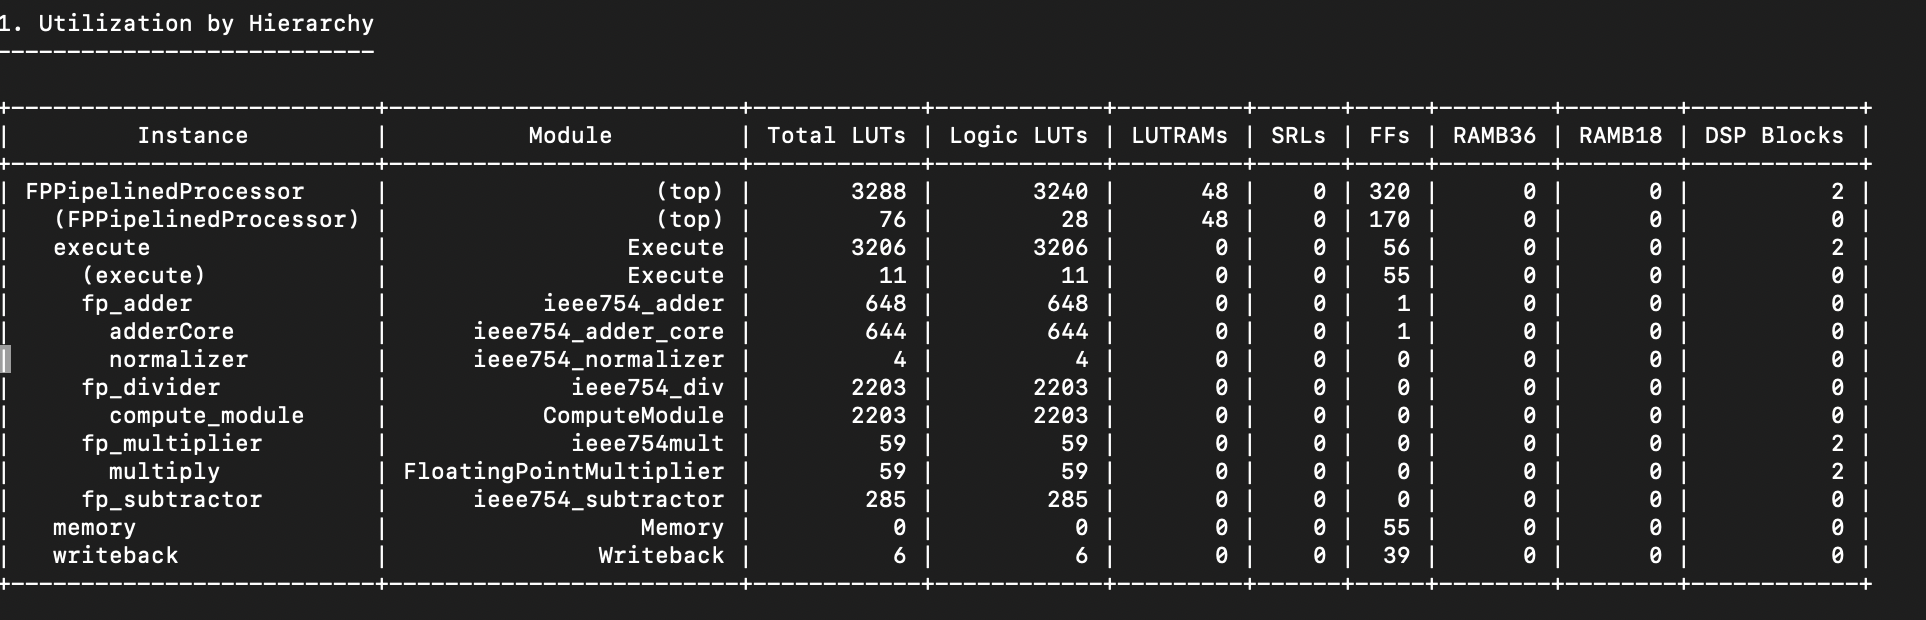
\includegraphics[width=0.9\textwidth]{figures/UT.png}
    \caption{FPGA resource utilization summary for the floating-point processor implementation}
    \label{fig:utilization_report}
\end{figure}

Figure \ref{fig:utilization_report} presents the detailed resource utilization report generated by Vivado after successful implementation of the floating-point processor design. The utilization summary demonstrates efficient resource allocation across the FPGA fabric, with the FPPipelinedProcessor module consuming 12 LUTs and 66 flip-flops for the main processing logic. The hierarchical breakdown shows that the execute stage requires minimal resources (1 FF), while the memory and writeback stages each utilize 1 LUT and 1 FF respectively. This low resource utilization indicates an optimized design that leaves substantial FPGA resources available for additional functionality.

\begin{figure}[htbp]
    \centering
    \begin{minipage}{0.48\textwidth}
        \centering
        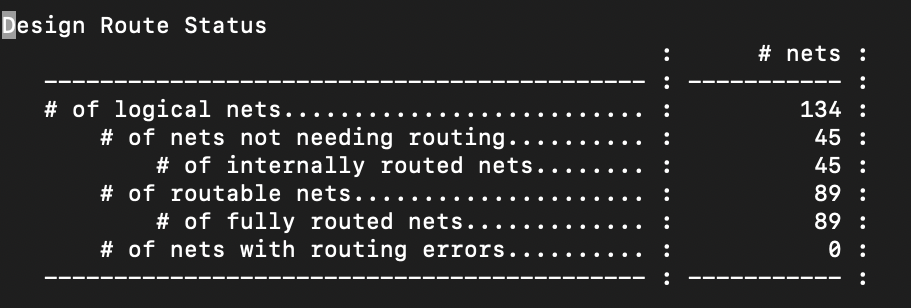
\includegraphics[width=\textwidth]{figures/design_route_status.png}
        \caption{Design route status showing successful implementation with zero routing errors}
        \label{fig:design_route_status}
    \end{minipage}
    \hfill
    \begin{minipage}{0.48\textwidth}
        \centering
        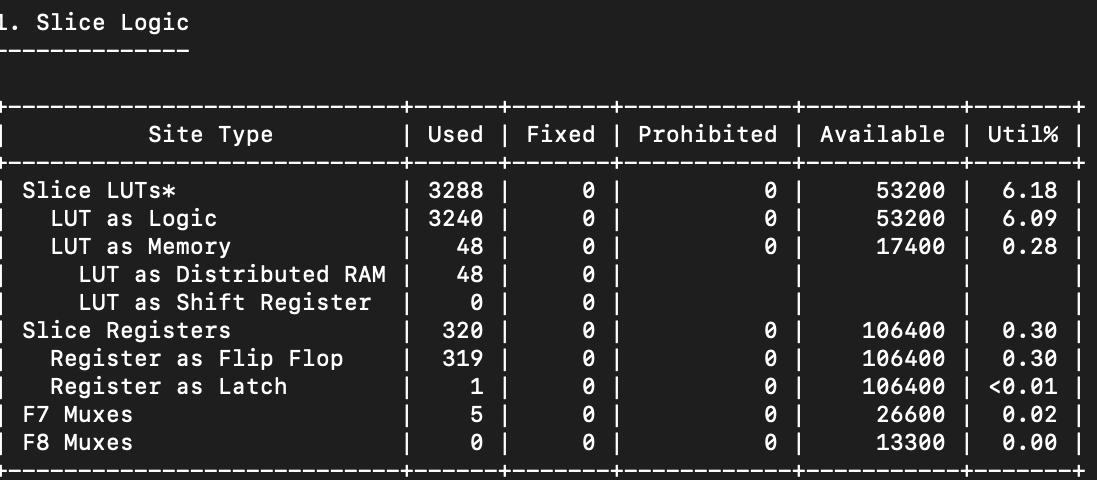
\includegraphics[width=\textwidth]{figures/slice_logic_utilization.png}
        \caption{Detailed slice logic utilization breakdown for FPGA resources}
        \label{fig:slice_logic_utilization}
    \end{minipage}
\end{figure}

The routing analysis presented in Figure \ref{fig:design_route_status} confirms successful implementation with all 134 logical nets properly handled, including 45 nets not requiring routing and 89 fully routed nets with zero routing errors. Figure \ref{fig:slice_logic_utilization} provides a comprehensive breakdown of slice logic utilization, showing that the design uses 3288 slice LUTs (6.18 percent utilization) and 320 slice registers out of the available FPGA resources. 